\let\negmedspace\undefined
\let\negthickspace\undefined
\documentclass[journal]{IEEEtran}
\usepackage[a5paper, margin=10mm, onecolumn]{geometry}
\usepackage{lmodern} 
\usepackage{tfrupee} 

\setlength{\headheight}{1cm} 
\setlength{\headsep}{0mm}     

\usepackage{gvv-book}
\usepackage{gvv}
\usepackage{cite}
\usepackage{amsmath,amssymb,amsfonts,amsthm}
\usepackage{algorithmic}
\usepackage{graphicx}
\usepackage{textcomp}
\usepackage{xcolor}
\usepackage{txfonts}
\usepackage{listings}
\usepackage{enumitem}
\usepackage{mathtools}
\usepackage{gensymb}
\usepackage{comment}
\usepackage[breaklinks=true]{hyperref}
\usepackage{tkz-euclide} 
\usepackage{listings}
\def\inputGnumericTable{}                                 
\usepackage[latin1]{inputenc}                                
\usepackage{color}                                            
\usepackage{array}                                            
\usepackage{longtable}                                       
\usepackage{calc}                                             
\usepackage{multirow}                                         
\usepackage{hhline}                                           
\usepackage{ifthen}                                           
\usepackage{lscape}
\begin{document}

\bibliographystyle{IEEEtran}
\vspace{3cm}

\title{2.2.21}
\author{AI25BTECH11028 - RAYIDI MANOHAR}
\maketitle
\bigskip
{\let\newpage\relax\maketitle}


\renewcommand{\thefigure}{\theenumi}
\renewcommand{\thetable}{\theenumi}
\setlength{\intextsep}{10pt} 


\numberwithin{equation}{enumi}
\numberwithin{figure}{enumi}
\renewcommand{\thetable}{\theenumi}


\textbf{Question}:
If the angle between two lines is $\pi/4$ and slope of one of the lines is $1/2$,find the slope of the other line.

\textbf{Solution:}

We know that,
The angle $\theta$ between $\vec{a},\vec{b}$, is given by 

\begin{align}
\cos \theta = \frac{\vec{a}^\top \vec{b}}{\|\vec{a}\| \|\vec{b}\|}
\end{align}


From the given Information,
Angle between the lines is $\pi/4$ 
let vector $\vec{A}$ be the line slope 1/2  and $\vec{B}$ be the line with slope $m_2$

\begin{align}
    \vec{A}=\myvec{1\\1/2} \\
    \vec{B}=\myvec{1\\m_2}
\end{align}

\begin{align}
    \cos{\pi/4} = \frac{\vec{A}^\top \vec{B}}{\|\vec{A}\| \|\vec{B}\|}
\end{align}

Now,
\begin{align}
       \vec{A}^\top \vec{B}&=\myvec{1\\1/2}^\top \myvec{1\\m_2}=1^2+m_2/2\\
\|\vec{A}\| &= \sqrt{1^2 + \left(\frac{1}{2}\right)^2} = \sqrt{1 + \frac{1}{4}} = \sqrt{\frac{5}{4}} = \frac{\sqrt{5}}{2} \\
\|\vec{B}\| &= \sqrt{1^2 + m_2^2} = \sqrt{1 + m_2^2}
\end{align}

From this,

\begin{align}
    \frac{1}{\sqrt{2}}*\frac{\sqrt{5}}{2}*\sqrt{1+m_2^2}=1+\frac{m_2}{2}\\
    \sqrt{5}*\sqrt{1+m_2^2}=\sqrt{2}(2+m_2)
\end{align}
 Now squaring on both sides;
\begin{align}
    5+5m_2^2=2(4+m_2^2+4m_2)\\
    3m_2^2-8m_2-3=0
\end{align}

Therefore,
\begin{align}
    m_2=3or-1/3
\end{align}
 \centering
    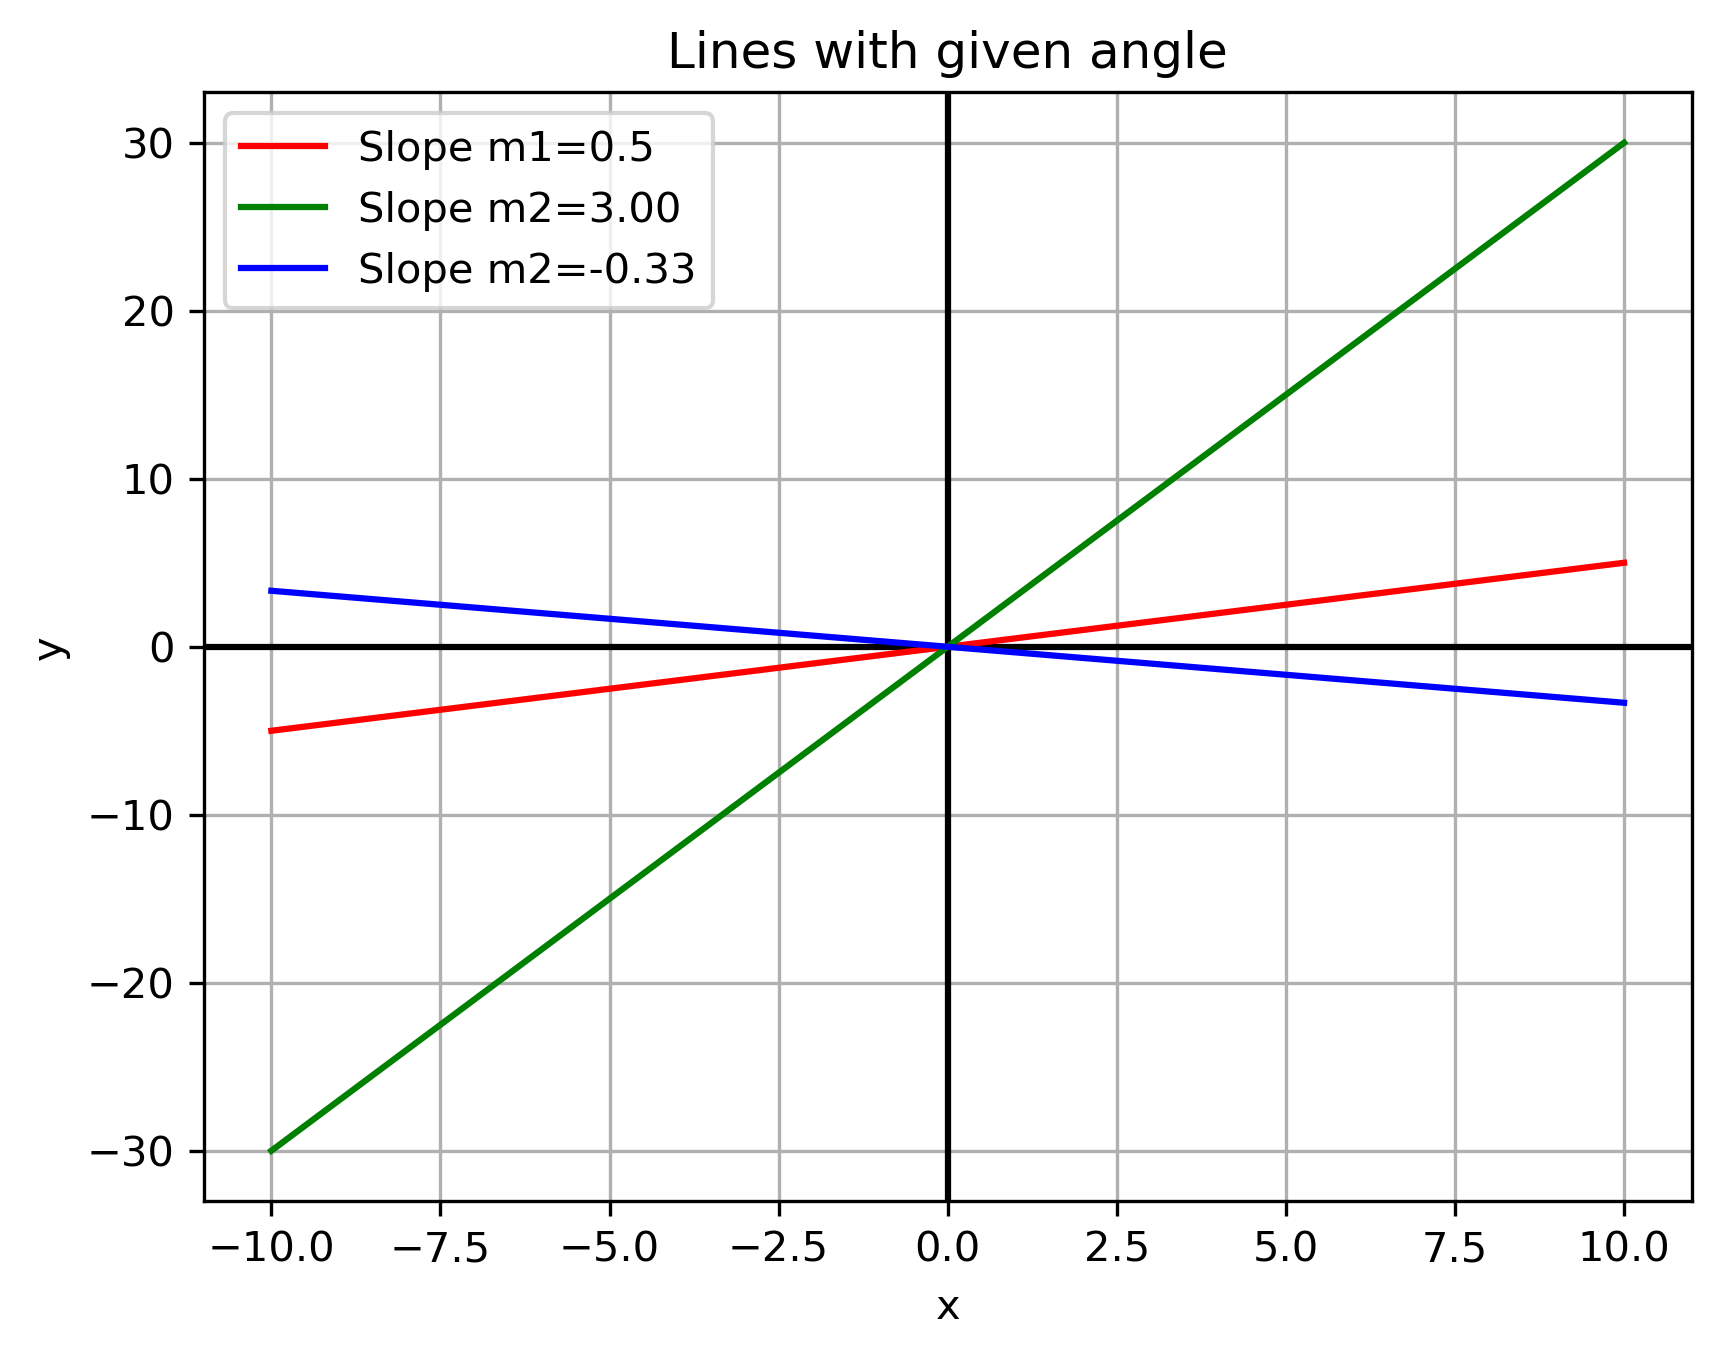
\includegraphics[width=\columnwidth, height=0.8\textheight, keepaspectratio]{figs/Figure_1.png}


\end{document}

